\documentclass[preprint,12pt]{elsarticle}
%DIF LATEXDIFF DIFFERENCE FILE
%DIF DEL /tmp/old-flat.tex   Mon Jan 26 18:50:04 2026
%DIF ADD /tmp/new-flat.tex   Mon Jan 26 18:49:53 2026







\usepackage{amssymb}
\usepackage{amsmath}
\usepackage{comment}
\usepackage{url}
\usepackage{hyperref}


\usepackage{tikz}
\usepackage[dvipsnames]{xcolor}
\usepackage{multirow}
\renewcommand{\paragraph}[1]{}
%DIF PREAMBLE EXTENSION ADDED BY LATEXDIFF
%DIF UNDERLINE PREAMBLE %DIF PREAMBLE
\RequirePackage[normalem]{ulem} %DIF PREAMBLE
\RequirePackage{color}\definecolor{RED}{rgb}{1,0,0}\definecolor{BLUE}{rgb}{0,0,1} %DIF PREAMBLE
\providecommand{\DIFaddtex}[1]{{\protect\color{blue}\uwave{#1}}} %DIF PREAMBLE
\providecommand{\DIFdeltex}[1]{{\protect\color{red}\sout{#1}}} %DIF PREAMBLE
%DIF SAFE PREAMBLE %DIF PREAMBLE
\providecommand{\DIFaddbegin}{} %DIF PREAMBLE
\providecommand{\DIFaddend}{} %DIF PREAMBLE
\providecommand{\DIFdelbegin}{} %DIF PREAMBLE
\providecommand{\DIFdelend}{} %DIF PREAMBLE
\providecommand{\DIFmodbegin}{} %DIF PREAMBLE
\providecommand{\DIFmodend}{} %DIF PREAMBLE
%DIF FLOATSAFE PREAMBLE %DIF PREAMBLE
\providecommand{\DIFaddFL}[1]{\DIFadd{#1}} %DIF PREAMBLE
\providecommand{\DIFdelFL}[1]{\DIFdel{#1}} %DIF PREAMBLE
\providecommand{\DIFaddbeginFL}{} %DIF PREAMBLE
\providecommand{\DIFaddendFL}{} %DIF PREAMBLE
\providecommand{\DIFdelbeginFL}{} %DIF PREAMBLE
\providecommand{\DIFdelendFL}{} %DIF PREAMBLE
%DIF HYPERREF PREAMBLE %DIF PREAMBLE
\providecommand{\DIFadd}[1]{\texorpdfstring{\DIFaddtex{#1}}{#1}} %DIF PREAMBLE
\providecommand{\DIFdel}[1]{\texorpdfstring{\DIFdeltex{#1}}{}} %DIF PREAMBLE
%DIF AMSMATHULEM PREAMBLE %DIF PREAMBLE
\makeatletter %DIF PREAMBLE
\let\sout@orig\sout %DIF PREAMBLE
\renewcommand{\sout}[1]{\ifmmode\text{\sout@orig{\ensuremath{#1}}}\else\sout@orig{#1}\fi} %DIF PREAMBLE
\makeatother %DIF PREAMBLE
%DIF COLORLISTINGS PREAMBLE %DIF PREAMBLE
\RequirePackage{listings} %DIF PREAMBLE
\RequirePackage{color} %DIF PREAMBLE
\lstdefinelanguage{DIFcode}{ %DIF PREAMBLE
%DIF DIFCODE_UNDERLINE %DIF PREAMBLE
  moredelim=[il][\color{red}\sout]{\%DIF\ <\ }, %DIF PREAMBLE
  moredelim=[il][\color{blue}\uwave]{\%DIF\ >\ } %DIF PREAMBLE
} %DIF PREAMBLE
\lstdefinestyle{DIFverbatimstyle}{ %DIF PREAMBLE
	language=DIFcode, %DIF PREAMBLE
	basicstyle=\ttfamily, %DIF PREAMBLE
	columns=fullflexible, %DIF PREAMBLE
	keepspaces=true %DIF PREAMBLE
} %DIF PREAMBLE
\lstnewenvironment{DIFverbatim}[1][]{\lstset{style=DIFverbatimstyle}}{} %DIF PREAMBLE
\lstnewenvironment{DIFverbatim*}[1][]{\lstset{style=DIFverbatimstyle,showspaces=true}}{} %DIF PREAMBLE
\lstset{extendedchars=\true,inputencoding=utf8}

%DIF END PREAMBLE EXTENSION ADDED BY LATEXDIFF

\begin{document}

\begin{frontmatter}





\title{DeXposure-FM: A Time-series, Graph Foundation Model on Credit Exposures and Stability on Decentralised Financial Networks}

\author[label1]{Aijie Shu}\author[label2]{Wenbin Wu}
\author[label3,label1]{Fengxiang He}\ead{F.He@ed.ac.uk}

\affiliation[label1]{organization={The Franc Team},
country={United Kingdom}}


\affiliation[label2]{organization={Cambridge Centre for Alternative Finance, Judge Business School, University of Cambridge},
country={United Kingdom}}

\affiliation[label3]{organization={School of Informatics, University of Edinburgh},
country={United Kingdom}}













\begin{abstract}
We introduce DeXposure-FM, to our best knowledge the first time-series, graph foundation model for measuring and forecasting inter-protocol credit exposures on decentralised financial networks. The model \DIFdelbegin \DIFdel{has an architecture of xxx}\DIFdelend \DIFaddbegin \DIFadd{uses a pre-trained GraphPFN encoder with task-specific prediction heads}\DIFaddend . The model is built over a large-scale dataset DeXposure, which reconstructs value-linked credit exposures (measured by Total Value Locked, TVL) and token flows across 4,300+ protocols on 602 blockchains, covering 24,300+ unique tokens over 2020--2025, totally over 43.7 million snapshots. DeXposure-FM is trained for the task of edge-level credit-exposure forecasting by an advanced optimiser, Sharpness-Aware Minimization (SAM), predicting the joint dynamics of (1) protocol-level TVL and flows, (2) the topology and weights of credit-exposure links, and (3) sector structure (lending, exchanges, asset management, bridges, stablecoins, etc.).

We evaluate DeXposure-FM on a suite of machine-learning benchmarks: (1) multi-step forecasting of edge-level exposures and network-level statistics, including concentration, density, and sector connectivity; (2) policy-relevant scenario analysis, where the model generates shock-consistent paths of losses and contagion during major stress events; and (3) imputation and denoising of missing or noisy exposures and TVL histories, with TVL-weighted error metrics and downstream performance on forecasting and link-prediction tasks. We compare DeXposure-FM to \DIFdelbegin \DIFdel{baselines including VAR models, low-rank factor models, }\DIFdelend \DIFaddbegin \DIFadd{graph-based baselines including frozen graph encoders }\DIFaddend and temporal graph neural networks.

On the financial economics front, we use the foundation model to construct dynamic measures of (1) protocol-level systemic importance, (2) sector-to-sector spillover indices, and (3) early-warning indicators based on shifts in network concentration and dependence on fragile collateral. We show how these AI-generated statistics can support macroprudential monitoring, DeFi-specific stress testing, and counterfactual policy evaluation (e.g., caps on bridges or leverage and alternative collateral rules), while also highlighting conditions under which foundation-model-based measures of digital financial infrastructure are robust, and where they call for cautious interpretation by regulators and central banks.





\end{abstract}



\begin{highlights}
\item Financial economics foundation model: We build DeXposure-FM, the first time-series, graph foundation model in DeFi and the wider financial economic space.

\item Financial economics / ML benchmarks: We show that DeXposure-FM produces competitive multi-step forecasts of edge-level exposures and network-level statistics (concentration, density, sector-to-sector links) relative to econometric and machine learning baselines (factor-VARs, temporal GNNs).

\item Economic measurement and systemic-risk statistics for DeFi: We use DeXposure-FM to derive richer systemic-risk measures: protocol-level systemic-importance scores, sectoral spillover indices, and early-warning indicators based on shifts in network structure and reliance on fragile collateral-providing information beyond standard size- and TVL-based metrics and supporting macroprudential surveillance and DeFi regulation.

\item Financial risk stress testing: Using the model, we generate shock-consistent scenarios for major DeFi stress events (e.g. stablecoin de-pegs, exchange failures) and quantify loss distributions, contagion paths, and the impact of counterfactual policy tools (leverage caps, collateral haircuts, bridge limits).
\end{highlights}

\begin{keyword}
Time-Series Analysis \sep Graph Tabular Model \sep Foundation Model \sep Credit Exposures \sep Financial Stability \sep Decentralised Finance \sep Financial Networks








\end{keyword}

\end{frontmatter}



\newpage
\tableofcontents

\section{Introduction}



Decentralised finance (DeFi) has emerged as an important and fast-evolving financial ecosystem, offering lending, trading, derivatives and payment-like services via smart contracts deployed across multiple blockchains \cite{Schar2021DeFi,Gogol2024SoKDeFi}. A defining feature of DeFi is composability: protocols routinely hold, lock, or accept tokens issued by other protocols as collateral, liquidity, or reserves. As a result, credit exposure is often implicit and token-mediated rather than expressed as bilateral contracts, creating a dense web of inter-protocol dependencies \cite{wu2025,Bertomeu2024}. When a token that is widely used as collateral or liquidity experiences a shock, through a price collapse, governance failure, exploit, or liquidation event; losses can propagate to protocols that rely on that token, potentially generating amplification and contagion across chains \cite{Aufiero2025,Gogol2024SoKDeFi}. 

Policy bodies have repeatedly highlighted that DeFi can replicate traditional financial functions while inheriting familiar vulnerabilities, leverage, liquidity and maturity transformation, operational fragilities, and interconnectedness, often in forms that can unwind abruptly because key risk-management processes are automated in code \cite{FSB2023,IOSCO2023DeFi}. In particular, collateralised lending protocols rely on oracles and liquidation mechanisms that can trigger rapid deleveraging and fire-sale dynamics when prices move sharply or data feeds are disrupted \cite{DuleyEtAl2023Oracle,SasiBrodeskyNassr2023DeFiLiquidations,TianZhu2025Liquidations}. Stablecoins are a central node in these dynamics: they serve as settlement assets and collateral across protocols, and their de-pegs and runs can transmit stress through both on-chain and off-chain channels \cite{KosseEtAl2023Stablecoin,AnaduEtAl2023StablecoinsMMF,ESRB2025}. Yet regulators and researchers emphasise persistent data gaps that hinder monitoring and the construction of standardised risk indicators for the DeFi ecosystem \cite{FSB2023,IOSCO2023DeFi}. This measurement gap is increasingly salient as links between crypto markets and the broader financial system deepen \cite{ESRB2025}.

Despite the importance, empirical work has been constrained by limited data and tools. DeFi exposures are not reported in standardized balance sheets; they must be reconstructed from on-chain states and transactions. Even when exposures can be estimated, they are (1) high-dimensional: there are millions of potential directed links, (2) nonstationary in terms of protocol upgrades, new assets, changing incentives, and (3) strongly heteroskedastic: regime shifts between calm and crisis. Classical time-series tools such as vector autoregressions (VARs) \citep{Sims1980} and low-rank factor methods \citep{StockWatson2002} provide strong baselines, but they struggle to represent the coupled evolution of \emph{node-level states} (e.g., total locked value in a protocol), \emph{edge-level exposures} (who is economically linked to whom, and with what weight), and \emph{meso-structure} (sectoral organization and its rewiring under stress). Meanwhile, modern graph neural networks (GNNs) \citep{KipfWelling2017,VelickovicEtAl2018} and temporal graph models for dynamic interaction data \citep{RossiEtAl2020TGN} offer expressive inductive biases, yet they are typically trained for a narrow task on a single dataset, rather than serving as reusable infrastructure across forecasting, scenario generation, and data repair.

To address this gap, we train \textbf{DeXposure-FM}, a time-series, graph foundation model for measuring and forecasting inter-protocol credit exposures in global decentralized financial networks. The model is trained on the \textbf{DeXposure} dataset, which reconstructs value-linked credit exposures and token flows across more than 4,300 protocols on 602 blockchains, covering over 24,300 tokens from 2020-2025, over 43.7 million weekly snapshots in total \cite{wu2025}. DeXposure operationalizes inter-protocol exposures by linking protocol balance-sheet dynamics (e.g., total value locked, TVL) to token- and sector-level structure, enabling a unified view of volumes, topology, and compositional risk. DeXposure-FM follows the foundation-model paradigm: it pretrains a general representation on heterogeneous data and reuses it across downstream tasks, a strategy that has proven effective in time-series and structured-data settings \cite{liang2024fmts,eremeev2025g2tfm}. 

The data is an evolving, weighted, directed multigraph whose nodes are protocols (and optionally protocol-token pairs) and whose edges represent economically meaningful exposure links inferred from value and flow relationships. The modeling challenge is not merely to predict edge weights; it is to learn the \emph{joint dynamics} of: (1) protocol-level TVL and token flows, (2) the topology and weights of exposure links, and (3) sector structure, including lending, exchanges, asset management, bridges, stablecoins, etc. These outputs map naturally to policy-relevant statistics: concentration, density, sector connectivity, and directional spillovers \citep{DieboldYilmaz2012}. In crises, the relevant question is not only ``what is the expected TVL tomorrow?'', but ``which parts of the network amplify shocks, and along which pathways does distress travel?'' \citep{EisenbergNoe2001,BattistonEtAl2012DebtRank}.
Because large models could overfit sharp minima that generalize poorly, we employ Sharpness-Aware Minimization (SAM) \citep{ForetEtAl2021SAM}, an advanced optimizer, which explicitly biases learning toward flatter regions in parameter space, provably leading to better generalizability.

We evaluate DeXposure-FM on a suite of machine-learning benchmarks tailored to economic measurement and risk analytics: (1) multi-step forecasting of edge-level exposures and network-level statistics (e.g., concentration, density, and sector connectivity), (2) policy-relevant scenario analysis by generating shock-consistent paths of losses and contagion around major stress events (e.g., stablecoin de-pegs and exchange failures), and (3) imputation and denoising of missing or noisy exposure and TVL histories using TVL-weighted metrics and downstream performance on forecasting and link-prediction tasks. Across tasks, we benchmark against \DIFdelbegin \DIFdel{classical econometric and latent-structure baselines (e.g., VAR and factor models) as well as }\DIFdelend \DIFaddbegin \DIFadd{graph-based baselines including frozen graph encoders and }\DIFaddend temporal graph neural networks. 

On the financial economics front, DeXposure-FM provides a generative measurement layer for macroprudential monitoring in digital financial infrastructure. We use the trained model to construct dynamic measures of protocol-level systemic importance, sector-to-sector spillover indices, and early-warning indicators based on shifts in network concentration and dependence on fragile collateral. These AI-generated statistics support DeFi-specific stress testing and counterfactual policy evaluation (e.g., caps on bridge exposures or leverage, and alternative collateral rules), while clarifying when model-based measures are robust and when they require cautious interpretation by regulators and central banks. By combining novel on-chain data with a multimodal foundation model, DeXposure-FM advances the measurement toolkit needed to understand systemic risk in DeFi and its interaction with the wider financial system \cite{naifar2025mapping,aufiero2025mapping}. \section{Related Works}







\subsection{Credit Risk Modeling in Traditional and Decentralized Finance}
In traditional finance, credit risk modeling spans both individual-default models and systemic network approaches.  Classical structural models (e.g., Merton) and reduced-form models quantify default probabilities of single entities, while network contagion models examine how defaults propagate through financial institutions.  For example, \cite{Dolfin2019} apply network epidemic models to credit contagion, highlighting how interconnected portfolios can amplify systemic credit risk.  
In decentralized finance, credit risk manifests differently, as loans are typically over-collateralized and mediated by smart contracts.  \cite{Bertomeu2024} propose simple aggregate risk measures for DeFi lending protocols, using only total deposits and borrowings, and report that systemic fragility surged around mid-2021 during crypto market turmoil.  Complementing these measures, \cite{wu2025} define inter-protocol credit exposures based on changes in Total Value Locked (TVL), enabling new graph-based analysis of DeFi credit networks.  Conceptual studies have begun to map TradFi and DeFi risks together: \cite{Aufiero2025} review systemic risk mechanisms, finding that while basic risk types (leverage, liquidity shocks, correlated exposures) are common to both systems, DeFi's algorithmic execution and composability lead to unique propagation channels.

\subsection{Machine Learning for Systemic Risk, Contagion, and Network Analysis}
Machine learning techniques are increasingly applied to systemic risk detection and contagion modeling.  Graph neural networks (GNNs) in particular leverage network structure to improve risk prediction.  \cite{Balmaseda2023} show that a GNN-based model dramatically outperforms traditional ML for classifying systemic importance of banks in simulated networks: GNNs achieved a 94\% higher correlation metric on average compared to standard ML classifiers.  Likewise, \cite{Gonon2024} integrate GNNs with explicit interbank liability networks, computing systemic risk measures as the minimum capital needed to secure the system.  Their framework effectively learns contagion channels (e.g., Eisenberg--Noe clearing) by incorporating graph-structured data into the risk aggregation function.  These modern ML approaches build on network science foundations.  Overall, machine-learning-driven network analysis enables end-to-end forecasting of systemic events, aiming to detect contagion pathways and provide early warnings for financial crises.

\subsection{Foundation Models in Finance and Economics}

Foundation models are increasingly penetrated into financial and economic domains by shifting the workflow from task-specific tools toward reusable representations learned from broad, heterogeneous data. Instead of fitting a separate model for each target, recent approaches pretrain large neural networks, mostly transformer variants, on massive data and then transfer them across domains and tasks via prompting or light adaptation \citep{AnsariEtAl2024Chronos,RasulEtAl2023LagLlama,DasEtAl2024TimesFM}. In parallel, an emerging policy-facing literature uses large language models to extract quantitative signals from narrative text (e.g., reports, releases, and news) and incorporate them into nowcasting pipelines, suggesting that relatively small but information-dense text sources can improve real-time prediction when combined with standard indicators \citep{deBondtSun2025ChatGPTNowcast,KwonEtAl2024BISLLMprimer,CarrieroEtAl2024MacroLLM}. Beyond ``pure'' time series, foundation-model architectures for structured data broaden the toolkit for financial applications: transformer-based models adapted to graph inputs, such as Graphormer \citep{Ying2021Graphormer}, augment self-attention with graph structural encodings (including spatial and centrality features), demonstrating the feasibility of large pretrained models on networks that resemble webs of financial contracts or cross-asset relationships. For tabular data, the Tabular Prior-Data Fitted Network (TabPFN) \citep{HollmannEtAl2025TabPFN} is pretrained on millions of synthetic tabular tasks and reports strong out-of-the-box performance on diverse benchmarks with up to 10,000 samples, while also supporting generative uses such as density estimation and data generation. 


%
 \section{Formalising Credit-Exposures on Decentralised Financial Networks}

A hallmark of decentralised finance is that protocols lock and issue tokens that circulate across multiple platforms.  When a lending protocol such as MakerDAO accepts wrapped ether (WETH) as collateral or a liquidity pool holds stablecoins minted by Circle or Tether, a web of implicit credit links arises: the value of one protocol’s liabilities depends on the solvency and liquidity of another.  Traditional financial network models highlight that interconnectedness can diversify risk but also create channels for contagion; the amplification or dampening of shocks depends on network structure, leverage, and recovery rates \cite{Glasserman2016}.  Early systemic‑risk research used clearing vectors to characterise interbank obligations and showed that fixed‑point algorithms can compute consistent payment outcomes even in the presence of cyclical interdependence \cite{EisenbergNoe2001}.  More recent work demonstrates that as networks become more complete, the stability of the system initially improves but may deteriorate beyond a critical threshold because dense interconnections propagate shocks \cite{Acemoglu2013}.  These insights motivate a rigorous formalisation of credit‑exposure in DeFi networks.

\subsection{Credit Exposure}

Let $X_G(q)$ denote the set of all tokens issued or generated by protocol $q$, and let $X_p(t)$ denote the set of tokens held (or locked) by protocol $p$ at time $t$.  Following \cite{wu2025}, we say that protocol $p$ has {credit exposure} to protocol $q$ at time~$t$ if the tokens it holds include at least one that was issued by $q$:
\begin{equation}
X_p(t)\cap X_G(q)\neq \varnothing.
\label{eq:credit-exposure-definition}
\end{equation}
In other words, $p$ holds a liability of $q$; if the tokens issued by $q$ lose value or become illiquid, then $p$ faces a corresponding loss.  This token‑mediated dependence generalises the notion of counterparty credit risk in traditional finance to decentralised platforms, where exposures arise not from explicit bilateral contracts but from the possession of tokenised claims.  The DeXposure dataset measures the dynamics of these relationships by reconstructing total value locked (TVL) time series for each protocol and tracking how the composition of tokens held by each protocol evolves over time.



\DIFdelbegin %DIFDELCMD < \begin{figure}[h]
%DIFDELCMD <     %%%
\DIFdelendFL \DIFaddbeginFL \begin{figure}[htbp]
    \DIFaddendFL \centering
    \DIFdelbeginFL %DIFDELCMD < \begin{tikzpicture}[node distance=3cm, auto]
%DIFDELCMD <         \tikzstyle{entity} = [rectangle, draw, fill=Apricot, minimum width=2cm, minimum height=1cm]
%DIFDELCMD <         \tikzstyle{balance} = [rectangle, draw, fill=SpringGreen, minimum width=3.8cm, minimum height=3cm]
%DIFDELCMD <     

%DIFDELCMD <         \node[entity] (user) at (0,2) {User};
%DIFDELCMD <         \node[entity] (weth) at (-4,0) {WETH Protocol};
%DIFDELCMD <         \node[entity] (maker) at (4,0) {MakerDAO};
%DIFDELCMD <         

%DIFDELCMD <         \node[balance] (balanceWETH) at (-4,-2.5) {
%DIFDELCMD <             \begin{tabular}{lr}
%DIFDELCMD <                 \textbf{WETH Protocol} & \\
%DIFDELCMD <                 Assets: & \\
%DIFDELCMD <                 ETH & \$100 \\
%DIFDELCMD <                 Liabilities: & \\
%DIFDELCMD <                 WETH & \$100
%DIFDELCMD <             \end{tabular}
%DIFDELCMD <         };
%DIFDELCMD <         \node[balance] (balanceMaker) at (4,-2.5) {
%DIFDELCMD <             \begin{tabular}{lr}
%DIFDELCMD <                 \textbf{MakerDAO} & \\
%DIFDELCMD <                 Assets: & \\
%DIFDELCMD <                 WETH & \$100 \\
%DIFDELCMD <                 Stability Buffer & \$-34 \\
%DIFDELCMD <                 Liabilities: & \\
%DIFDELCMD <                 DAI & \$66 \\
%DIFDELCMD <             \end{tabular}
%DIFDELCMD <         };
%DIFDELCMD <     

%DIFDELCMD <         \draw[->, thick] (user) to[bend left=30] node[above, midway] {ETH \$100} (weth);
%DIFDELCMD <         \draw[->, thick] (weth) to[bend left=30] node[below, midway] {WETH \$100} (user);
%DIFDELCMD <         \draw[->, thick] (user) to[bend right=30] node[above, midway] {WETH \$100} (maker);
%DIFDELCMD <         \draw[->, thick] (maker) to[bend right=30] node[below, midway] {DAI \$66} (user);
%DIFDELCMD < 

%DIFDELCMD <     \end{tikzpicture}
%DIFDELCMD <     %%%
\DIFdelendFL \DIFaddbeginFL 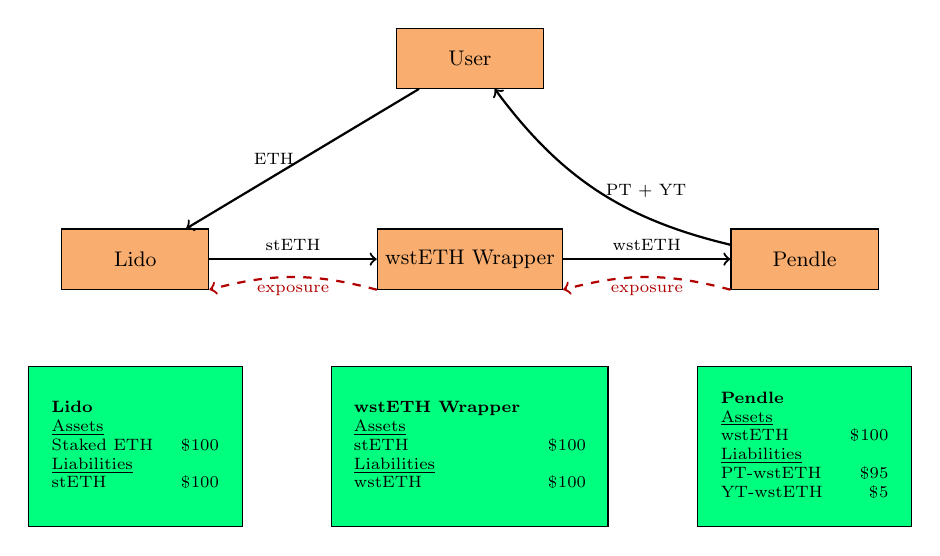
\begin{tikzpicture}[node distance=2.5cm, auto, scale=0.85, transform shape]
        \tikzstyle{entity} = [rectangle, draw, fill=Apricot, minimum width=2.2cm, minimum height=0.9cm, font=\small]
        \tikzstyle{balance} = [rectangle, draw, fill=SpringGreen, minimum width=3.2cm, minimum height=2.4cm, font=\scriptsize]
        \tikzstyle{exposure} = [->, thick, dashed, red!70!black]

\node[entity] (user) at (0,3) {User};

\node[entity] (lido) at (-5,0) {Lido};
        \node[entity] (wrapper) at (0,0) {wstETH Wrapper};
        \node[entity] (pendle) at (5,0) {Pendle};

\node[balance] (balanceLido) at (-5,-2.8) {
            \begin{tabular}{lr}
                \textbf{Lido} & \\
                \underline{Assets} & \\
                Staked ETH & \$100 \\
                \underline{Liabilities} & \\
                stETH & \$100
            \end{tabular}
        };
        \node[balance] (balanceWrapper) at (0,-2.8) {
            \begin{tabular}{lr}
                \textbf{wstETH Wrapper} & \\
                \underline{Assets} & \\
                stETH & \$100 \\
                \underline{Liabilities} & \\
                wstETH & \$100
            \end{tabular}
        };
        \node[balance] (balancePendle) at (5,-2.8) {
            \begin{tabular}{lr}
                \textbf{Pendle} & \\
                \underline{Assets} & \\
                wstETH & \$100 \\
                \underline{Liabilities} & \\
                PT-wstETH & \$95 \\
                YT-wstETH & \$5
            \end{tabular}
        };

\draw[->, thick] (user) -- node[left, font=\scriptsize] {ETH} (lido);
        \draw[->, thick] (lido) -- node[above, font=\scriptsize] {stETH} (wrapper);
        \draw[->, thick] (wrapper) -- node[above, font=\scriptsize] {wstETH} (pendle);
        \draw[->, thick] (pendle) to[bend left=20] node[right, font=\scriptsize] {PT + YT} (user);

\draw[exposure] (pendle.south west) to[bend right=15] node[below, font=\scriptsize, text=red!70!black] {exposure} (wrapper.south east);
        \draw[exposure] (wrapper.south west) to[bend right=15] node[below, font=\scriptsize, text=red!70!black] {exposure} (lido.south east);

    \end{tikzpicture}
    \DIFaddendFL \caption{\DIFdelbeginFL \DIFdelFL{Credit Exposure Example: WETH Wrapping and Overcollateralized DAI Generation}\DIFdelendFL \DIFaddbeginFL \DIFaddFL{Multi-layer credit exposure in DeFi}\DIFaddendFL . \DIFdelbeginFL \DIFdelFL{User wraps }\DIFdelendFL \DIFaddbeginFL \DIFaddFL{A user stakes }\DIFaddendFL ETH \DIFdelbeginFL \DIFdelFL{to WETH}\DIFdelendFL \DIFaddbeginFL \DIFaddFL{with Lido}\DIFaddendFL , \DIFdelbeginFL \DIFdelFL{then uses WETH as collateral to generate DAI from MakerDAO}\DIFdelendFL \DIFaddbeginFL \DIFaddFL{receiving stETH}\DIFaddendFL , \DIFaddbeginFL \DIFaddFL{which is wrapped into wstETH and deposited into Pendle. Each protocol holds the liability of the preceding one, }\DIFaddendFL creating \DIFaddbeginFL \DIFaddFL{a chain of }\DIFaddendFL credit \DIFdelbeginFL \DIFdelFL{exposure }\DIFdelendFL \DIFaddbeginFL \DIFaddFL{exposures }\DIFaddendFL from \DIFdelbeginFL \DIFdelFL{MakerDAO }\DIFdelendFL \DIFaddbeginFL \DIFaddFL{Pendle }\DIFaddendFL to \DIFdelbeginFL \DIFdelFL{the WETH protocol}\DIFdelendFL \DIFaddbeginFL \DIFaddFL{Lido}\DIFaddendFL .}
    \label{fig:exposure_example}
\end{figure}

\DIFaddbegin \noindent \DIFaddend Figure~\ref{fig:exposure_example} \DIFdelbegin \DIFdel{(reproduced from \mbox{%DIFAUXCMD
\cite{wu2025}}\hskip0pt%DIFAUXCMD
) }\DIFdelend illustrates how a \DIFdelbegin \DIFdel{simple }\DIFdelend \DIFaddbegin \DIFadd{single }\DIFaddend user transaction creates a \DIFdelbegin \DIFdel{chain of exposures}\DIFdelend \DIFaddbegin \DIFadd{multi-layer chain of credit exposures in DeFi}\DIFaddend .  A user \DIFdelbegin \DIFdel{wraps ether (ETH ) into WETH via the WETH protocoland then deposits WETH into MakerDAO to generate the stablecoin DAI.
In balance‑sheet terms, the WETH protocol holds ETH as assets and issues WETH }\DIFdelend \DIFaddbegin \DIFadd{deposits ETH into Lido, a liquid staking protocol, and receives stETH, a rebasing token that accrues staking rewards.  The stETH is then wrapped into wstETH, a non-rebasing representation that is more compatible with DeFi protocols.  Finally, wstETH is deposited into Pendle, a yield-tokenisation protocol that splits the asset into a principal token PT-wstETH and a yield token YT-wstETH, allowing users to trade fixed and variable yield separately.
}

\DIFadd{In balance-sheet terms, Lido holds staked ETH with validators and issues stETH }\DIFaddend as liabilities, \DIFdelbegin \DIFdel{while MakerDAO holds WETH as collateral and issues DAI as liabilities.  Because MakerDAO’s assets include WETH, there is credit exposure from MakerDAO to the WETH protocol; a failure or devaluation of WETH would erode MakerDAO’s collateral}\DIFdelend \DIFaddbegin \DIFadd{the wstETH wrapper holds stETH and issues wstETH, and Pendle holds wstETH and issues the PT and YT pair.  Because each protocol's assets consist of tokens issued by the preceding protocol, a chain of credit exposures emerges: Pendle has exposure to the wstETH wrapper, which in turn has exposure to Lido.  If Lido experienced a slashing event or stETH de-pegged from ETH, the losses would cascade through wstETH and into Pendle, affecting PT and YT holders}\DIFaddend .  This example \DIFdelbegin \DIFdel{shows }\DIFdelend \DIFaddbegin \DIFadd{demonstrates }\DIFaddend that DeFi exposures are inherently \DIFdelbegin \DIFdel{multi‑layered: a single wrapped token can create a cascade of dependencies across protocols and chains}\DIFdelend \DIFaddbegin \DIFadd{multi-layered, as liquid staking, wrapping, and yield tokenisation compound into complex dependency structures that the DeXposure dataset aims to capture}\DIFaddend .

\subsection{Mapping Tokens to Issuing Protocols}

To operationalise \eqref{eq:credit-exposure-definition}, we must determine which protocol issues each token and thus identify the direction of exposure.  Let $\mathcal{P}$ denote the set of all protocols and $\mathcal{C}$ the set of blockchains.  For each token $\sigma$ appearing in protocol $p$, a \textbf{mapping function} $M(\sigma)$ returns the protocol $q$ that issues or manages $\sigma$.  The DeXposure dataset constructs $M$ using a fall‑back procedure:
\begin{enumerate}
  \item \textbf{Metadata lookup:} Tokens are directly matched to issuing protocols using metadata from DefiLlama when available.
  \item \textbf{Manual mapping:} For tokens with high TVL that lack metadata links, researchers manually assign the issuing protocol based on documentation and expert knowledge.
  \item \textbf{Text‑vector similarity:} For remaining tokens, the text descriptions of tokens and protocols are vectorised via the term frequency–inverse document frequency (TF--IDF) representation \cite{Qaiser2018}.  Cosine similarity scores between token and protocol vectors determine the best match, and tokens are mapped to the protocol with the highest similarity score exceeding a threshold $\theta$.
  \item \textbf{Primary market tokens:} If none of the above methods yields a mapping, the token is treated as its own protocol (e.g., WETH).
\end{enumerate}
This mapping ensures that token flows between protocols can be attributed to changes in credit exposure with respect to the correct issuing protocol, even when tokens are bridged across chains or wrapped by multiple platforms.

\subsection{Network Representation and Value Flows}

Credit exposures over a discrete time interval $\tau = t_2 - t_1$ are represented by a weighted directed graph $G_\tau = (P_\tau, E_\tau)$, where $P_\tau$ is the set of active protocols and $E_\tau$ is the set of directed edges.  Each vertex $p\in P_\tau$ is assigned a \textbf{node weight} equal to the value of assets it holds at the end of the interval:
\begin{equation}
w_\tau(p) = \sum_{\sigma\in X_p(t_1)\cap X_p(t_2)} v_{t_2,\sigma},
\label{eq:node-weight}
\end{equation}
where $v_{t_2,\sigma}$ is the USD value of token $\sigma$ at time $t_2$.  Nodes with negligible weight (below a threshold $\theta$) can be pruned for clarity.  To define the \textbf{edge weight} from protocol $p$ to protocol $q$, we first compute the value flow for each token $\sigma$:
\begin{equation}
F^{\sigma}_{p q,\tau} =
\begin{cases}
\max\bigl(0,\, -\Delta S^{\sigma}_{p,\tau}\bigr), & \text{if } \Delta S^{\sigma}_{p,\tau} < 0,\\
\max\bigl(0,\,\Delta S^{\sigma}_{q,\tau}\bigr), & \text{if } \Delta S^{\sigma}_{q,\tau} \ge 0,
\end{cases}
\label{eq:value-flow}
\end{equation}
where $\Delta S^{\sigma}_{p,\tau}=v_{p,t_2}^{\sigma}-v_{p,t_1}^{\sigma}$ is the change in the USD value of token $\sigma$ held by protocol $p$ over the interval.  Equation~\eqref{eq:value-flow} captures the intuition that if $p$ decreases its holdings of $\sigma$ and $q$ increases theirs, then $\sigma$ has flowed from $p$ to $q$; negative flows are reversed so that all flows are non‑negative.  The \textbf{edge weight} $w_\tau(e_{p q})$ is the sum of flows for all tokens that map to the issuing protocol $q$:
\begin{equation}
w_\tau(e_{p q}) = \sum_{\sigma \in X_{p q, \tau}} F^{\sigma}_{p q,\tau},
\label{eq:edge-weight}
\end{equation}
where $X_{p q,\tau}$ denotes the set of tokens with issuing protocol $q$ that move from $p$ to $q$ over $\tau$.  A positive edge weight indicates increasing exposure from $p$ to $q$.  For single‑token protocols, the flow of that token equals the edge weight.

Algorithm~1 in \cite{wu2025} describes a procedure for constructing $G_\tau$ from raw token‑protocol‑chain mappings.  In summary, one aggregates token holdings at the start and end of the interval, computes node weights, discards nodes below a threshold, and then computes edge weights by summing positive flows; negative flows are reversed to ensure all weights are non‑negative.  The resulting time‑indexed sequence of graphs captures the evolving structure of credit dependencies in the DeFi ecosystem.

\subsection{Discussion and links to systemic‑risk theory}

The above formalism bridges decentralised finance with established theories of financial networks.  By modelling credit exposures as weighted directed graphs derived from token flows, it becomes possible to apply systemic‑risk measures, such as centrality metrics, contagion indices, and stress tests, developed for interbank networks to DeFi.  Classical models show that fixed‑point algorithms can compute consistent clearing payments for interbank systems with cyclic obligations \cite{EisenbergNoe2001}, and that network structures can either buffer or amplify shocks depending on leverage and liquidity \cite{Glasserman2016}.  \cite{Acemoglu2013} further demonstrate that more complete networks initially enhance stability by distributing losses across many counterparties, but beyond a critical density the same interconnections propagate shocks and increase systemic fragility.  In the DeFi context, our graph formalisation reveals similar trade‑offs: diversifying collateral across multiple protocols may reduce reliance on any single issuer, yet highly interconnected protocols could become conduits for contagion if a stablecoin or wrapped token suffers a de‑peg or exploit.

This mathematical framework provides the foundation for the downstream tasks tackled by DeXposure‑FM.  Forecasting future node and edge weights, stress‑testing scenarios under shocks to token values, and imputing missing TVL data all rely on accurate representations of credit exposure.  Moreover, the network perspective aligns with macroprudential policy goals: regulators can monitor systemic importance and spillover risks by examining the temporal evolution of $G_\tau$, and researchers can evaluate how proposed protocol designs or regulatory interventions would reshape the exposure network.  As decentralised finance continues to grow and integrate with the broader financial system, rigorous formalisation and measurement of credit exposure will be essential for safeguarding stability and fostering responsible innovation. \section{DeXposure-FM: Architecture, Data, and Training}

This section introduces our DeXposure-FM, including its architecture, preparation of data, and the training process. The code is available at \url{https://github.com/EVIEHub/DeXposure-FM}.




\subsection{DeXposure-FM Architecture}
\label{sec:dexposure-fm-architecture}

DeXposure-FM leverages a pre-trained graph-tabular foundation model (GraphPFN) as its core encoder, which internally fuses graph structure and tabular node features. The model is designed to support three downstream objectives: (1) multi-step forecasting of edge weights and network statistics; (2) policy-relevant shock analysis on historical stress events; and (3) imputation of missing edges.

\subsubsection{Inputs and notation (aligned with the DeXposure construction)}
Let $t\in\mathcal{T}$ denote discrete observation times and let $\tau = t_2-t_1$ be a discrete interval between consecutive times.
For each interval $\tau$ we construct a weighted directed graph snapshot
\begin{equation}
G_{\tau}=(\mathcal{P}_{\tau},\mathcal{E}_{\tau}),
\end{equation}
where $\mathcal{P}_{\tau}$ is the set of protocols and $\mathcal{E}_{\tau}$ is the set of directed exposure links.
Node weights are given by $w_{\tau}(p)$ (the protocol's end-of-interval stock) as in Eq.~\eqref{eq:node-weight}, and edge weights are given by $w_{\tau}(e_{pq})$ (the change in credit exposure from $p$ to issuing protocol $q$ over $\tau$) as in Eq.~\eqref{eq:edge-weight}, where token-level value flows $F^{\sigma}_{pq,\tau}$ are defined by Eq.~\eqref{eq:value-flow}. Credit exposure exists when $X_p(t)\cap X_G(q)\neq\varnothing$ (Eq.~\eqref{eq:credit-exposure-definition}).

For each protocol $p$ we form the following inputs:
\begin{itemize}
  \item \textbf{Graph snapshot:} $G_{\tau}$ with node features including $w_{\tau}(p)$ and edge features including $w_{\tau}(e_{pq})$ (and optional attributes such as token class or sector pair).
  \item \textbf{Tabular node features:} $\mathbf{x}^{\mathrm{tab}}_{p}$ contains protocol descriptors including:
  \begin{itemize}
    \item Log-scaled TVL: $\log(1 + w_{\tau}(p))$
    \item Number of token types held
    \item Maximum token share (concentration measure)
    \item Token composition entropy
    \item Protocol category (one-hot encoded, $\sim$15 classes)
  \end{itemize}
\end{itemize}

\subsubsection{Graph-Tabular Encoder}
We employ GraphPFN \cite{eremeev2025g2tfm}, a pre-trained graph-tabular foundation model based on Transformer architecture, as our core encoder. GraphPFN jointly processes graph structure and tabular node features through multi-head self-attention with graph structure injection:
\begin{equation}
\{\mathbf{h}_{p,\tau}\}_{p\in\mathcal{P}_{\tau}} = E_{\mathrm{GraphPFN}}\!\left(G_{\tau}, \{\mathbf{x}^{\mathrm{tab}}_{p}\}_{p\in\mathcal{P}_{\tau}}\right),
\end{equation}
where $\mathbf{h}_{p,\tau}\in\mathbb{R}^d$ is the $d$-dimensional node embedding for protocol $p$ at time $\tau$.

The encoder can be operated in two modes:
\begin{itemize}
  \item \textbf{Frozen probing:} Encoder weights are frozen; only task heads are trained. This measures the transferability of pre-trained representations.
  \item \textbf{Fine-tuned:} End-to-end training with differential learning rates---lower rate ($\eta/10$) for the pre-trained backbone and higher rate ($\eta$) for task-specific heads.
\end{itemize}

\subsubsection{Task Heads}
\paragraph{(1) Multi-step forecasting.}
For horizon $h\in\{1,3,7,14\}$ weeks, we predict future edge existence and weights. The link scorer uses a Hadamard-product MLP architecture:
\begin{align}
\mathbf{f}_{pq} &= [\mathbf{h}_{p,\tau}; \mathbf{h}_{q,\tau}; \mathbf{h}_{p,\tau}\odot\mathbf{h}_{q,\tau}; |\mathbf{h}_{p,\tau}-\mathbf{h}_{q,\tau}|],\\
(\widehat{y}^{\mathrm{exist}}_{pq}, \widehat{w}_{\tau+h}(e_{pq})) &= \mathrm{MLP}_{\mathrm{link}}(\mathbf{f}_{pq}),
\end{align}
where $\widehat{y}^{\mathrm{exist}}_{pq}\in(0,1)$ is the predicted probability of edge existence, and $\widehat{w}_{\tau+h}(e_{pq})$ is the predicted edge weight (log-scaled).

For node-level prediction, we forecast the log-change in protocol TVL:
\begin{equation}
\widehat{\Delta}_{p,\tau+h} = \mathrm{MLP}_{\mathrm{node}}(\mathbf{h}_{p,\tau}),
\end{equation}
where $\widehat{\Delta}_{p,\tau+h} = \log(1+w_{\tau+h}(p)) - \log(1+w_{\tau}(p))$ for protocols $p\in\mathcal{P}_{\tau}\cap\mathcal{P}_{\tau+h}$.

Network-level statistics (concentration, density, sector connectivity) are obtained by applying deterministic functionals to the predicted graph $\widehat{G}_{\tau+h}$.

\paragraph{(2) Shock analysis.}
We evaluate model performance during extreme market events---specifically the Terra/Luna collapse (2022-05-09) and FTX collapse (2022-11-07). For each event, we examine a window around the shock date to assess:
\begin{itemize}
  \item Network structure changes (TVL, edge count, Gini, HHI)
  \item Model prediction performance degradation
  \item Early warning signal detection capability
\end{itemize}

\paragraph{(3) Imputation.}
We evaluate the model's ability to reconstruct missing edges under random masking. Edges are masked at rates $\{10\%, 20\%, 30\%\}$ following a Missing Completely at Random (MCAR) mechanism, and we report reconstruction quality via AUPRC and weight MAE.

\begin{comment}
    
\begin{figure}[t]
\centering
\begin{tikzpicture}[
  font=\footnotesize,
  scale=0.88, transform shape,
  box/.style={draw, rounded corners, align=center, minimum width=3.0cm, minimum height=0.9cm},
  sbox/.style={draw, rounded corners, align=center, minimum width=2.75cm, minimum height=0.82cm},
  arrow/.style={-Latex, thick},
  node distance=0.5cm and 0.85cm
]
\node[box] (tabin) {Tabular node features\\ $\mathbf{x}^{\mathrm{tab}}_{p}$};
  \node[box, below=of tabin] (graphin) {Exposure graph snapshot\\ $G_{\tau}=(\mathcal{P}_{\tau},\mathcal{E}_{\tau})$\\ Node: $w_{\tau}(p)$, Edge: $w_{\tau}(e_{pq})$};

\node[sbox, right=1.5cm of graphin] (egraph) {Pre-trained\\GraphPFN encoder\\ $E_{\mathrm{GraphPFN}}$};

\node[sbox, right=1.3cm of egraph] (embed) {Node embeddings\\ $\mathbf{h}_{p,\tau}$};

\node[sbox, right=1.2cm of embed] (forecast) {Forecasting head\\ $\widehat{w}_{\tau+h}(e_{pq}),\,\widehat{\Delta}_{p,\tau+h}$};
  \node[sbox, above=0.55cm of forecast] (shock) {Shock analysis\\ Terra/FTX events};
  \node[sbox, below=0.55cm of forecast] (impute) {Imputation\\ MCAR masking};

\draw[arrow] (tabin.east) -- ++(0.55,0) |- (egraph.west);
  \draw[arrow] (graphin) -- (egraph);

  \draw[arrow] (egraph) -- (embed);
  \draw[arrow] (embed) -- (forecast);

  \draw[arrow] (embed.east) -- ++(0.3,0) |- (shock.west);
  \draw[arrow] (embed.east) -- ++(0.3,0) |- (impute.west);

\node[draw, dashed, rounded corners, fit=(tabin)(graphin), inner sep=6pt, label={[align=center]above:Inputs}] {};
\end{tikzpicture}
\caption{DeXposure-FM architecture aligned with the DeXposure exposure-graph construction. The model uses a pre-trained GraphPFN encoder to jointly process graph structure and tabular node features, producing node embeddings $\mathbf{h}_{p,\tau}$ that support multi-step forecasting, shock analysis, and imputation tasks.}
\label{fig:dexposure-fm-architecture}
\end{figure}

\end{comment}
 \subsection{Training Pipeline}
\label{sec:training}

This section describes the training pipeline for DeXposure-FM. All graph and flow notation follows Section~\ref{sec:formalisation}.

\subsubsection{Training Data Preparation}

For each discrete interval $\tau$ we construct a weighted directed snapshot $G_{\tau}=(\mathcal P_{\tau},\mathcal E_{\tau})$ with node weights $w_{\tau}(p)$ and edge weights $w_{\tau}(e_{pq})$. We form training examples indexed by an anchor time $\tau$:
\begin{equation}
G_{\tau} \;\longrightarrow\; G_{\tau+h}, \quad h \in \{1, 3, 7, 14\},
\end{equation}
where the model predicts the graph state at horizon $h$ given the current snapshot.

For each protocol $p\in\mathcal P_{\tau}$ we provide tabular node features $\mathbf x^{\mathrm{tab}}_{p}$ (log-scaled TVL, token count, concentration measures, category) along with the graph structure $G_{\tau}$.

\paragraph{Time-based expanding window splits.}
We use expanding window walk-forward validation to ensure that all test targets occur strictly after the training window, thereby avoiding look-ahead bias. The training window expands over time while validation and test windows remain fixed.

\paragraph{Negative sampling.}
For edge existence prediction, we sample negative edges uniformly from the complement of the positive edge set, with a negative-to-positive ratio of 5:1.

\subsubsection{Training Modes}

We support two training modes for the GraphPFN encoder (the ROLAND baseline is trained from scratch as described in Section~\ref{sec:evaluation}):

\paragraph{Frozen probing.}
We freeze the pre-trained GraphPFN encoder and train only the task-specific heads (link scorer and node predictor). This setting measures the transferability of pre-trained representations to the DeFi exposure domain without modifying the backbone.

\paragraph{Fine-tuning.}
We perform end-to-end training with differential learning rates:
\begin{itemize}
  \item Pre-trained backbone: $\eta_{\text{backbone}} = \eta / 10$ (lower rate to preserve pre-trained knowledge)
  \item Task-specific heads: $\eta_{\text{heads}} = \eta$ (higher rate for new parameters)
\end{itemize}

\subsubsection{Loss Functions}
\label{sec:training:loss}

We train DeXposure-FM with a multi-task objective that combines three core prediction losses: edge existence, edge weight, and node TVL change prediction.

\paragraph{Edge existence loss (link prediction).}
We predict edge existence $\widehat{y}^{\mathrm{exist}}_{pq} \in (0,1)$ using binary cross-entropy with positive class weighting to handle class imbalance:
\begin{equation}
\mathcal L_{\mathrm{exist}} = \sum_{(p,q) \in \mathcal S_{\tau+h}} \mathrm{BCE}\bigl(\widehat{y}^{\mathrm{exist}}_{pq}, y^{\mathrm{exist}}_{pq}; w_{\mathrm{pos}}\bigr),
\label{eq:loss-exist}
\end{equation}
where $\mathcal S_{\tau+h}$ includes both positive edges from $\mathcal E_{\tau+h}$ and sampled negative edges (5:1 ratio), and $w_{\mathrm{pos}}$ is the positive class weight matching the negative sampling ratio.

\paragraph{Edge weight loss.}
For positive edges, we predict log-scaled edge weights using Smooth L1 loss:
\begin{equation}
\mathcal L_{\mathrm{weight}} = \sum_{(p,q) \in \mathcal E_{\tau+h}} \mathrm{SmoothL1}\bigl(\log(1+\widehat{w}_{\tau+h}(e_{pq})) - \log(1+w_{\tau+h}(e_{pq}))\bigr).
\label{eq:loss-weight}
\end{equation}
The log transformation $\log(1+\cdot)$ compresses the heavy-tailed distribution of exposures.

\paragraph{Node prediction loss.}
We predict the log-change in protocol TVL:
\begin{equation}
\mathcal L_{\mathrm{node}} = \sum_{p \in \mathcal P_{\tau} \cap \mathcal P_{\tau+h}} \mathrm{SmoothL1}\bigl(\widehat{\Delta}_{p,\tau+h} - \Delta_{p,\tau+h}\bigr),
\label{eq:loss-node}
\end{equation}
where $\Delta_{p,\tau+h} = \log(1+w_{\tau+h}(p)) - \log(1+w_{\tau}(p))$ is the ground-truth log-change in TVL.

\paragraph{Overall objective.}
The training objective combines the three core losses:
\begin{equation}
\mathcal L = \lambda_{\mathrm{exist}} \mathcal L_{\mathrm{exist}} + \lambda_{\mathrm{weight}} \mathcal L_{\mathrm{weight}} + \lambda_{\mathrm{node}} \mathcal L_{\mathrm{node}},
\label{eq:loss-total}
\end{equation}
with weights $\lambda_{\mathrm{exist}} = 2.0$, $\lambda_{\mathrm{weight}} = 0.5$, $\lambda_{\mathrm{node}} = 0.4$. Edge existence receives the highest weight as it is the primary task for link prediction; edge weight and node prediction provide complementary supervision for learning meaningful exposure representations.

\subsubsection{Optimizer and Schedule}

\paragraph{Optimizer.}
We use Adam with $\beta_1=0.9$, $\beta_2=0.999$, and learning rate $\eta = 5 \times 10^{-4}$.

\paragraph{Differential learning rates.}
For fine-tuning, we apply differential learning rates across parameter groups:
\begin{itemize}
  \item GraphPFN encoder: $\eta \times 0.1 = 5 \times 10^{-5}$ (to preserve pre-trained knowledge)
  \item Task-specific heads: $\eta = 5 \times 10^{-4}$
\end{itemize}

\paragraph{Training details.}
We train for up to 20 epochs with early stopping (patience=3) based on validation AUPRC. Gradient clipping ($\|\nabla\|_2 \le 1.0$) is applied for stability.

\begin{table}[t]
\centering
\small
\setlength{\tabcolsep}{6pt}
\renewcommand{\arraystretch}{1.05}
\begin{tabular}{ll}
\hline
\textbf{Hyperparameter} & \textbf{Value} \\
\hline
Data granularity & Weekly snapshots \\
Forecast horizons $h$ & $\{1, 3, 7, 14\}$ weeks \\
Negative sampling ratio & 5:1 (neg:pos) \\
Optimizer & Adam ($\beta_1=0.9$, $\beta_2=0.999$) \\
Learning rate (heads) & $5 \times 10^{-4}$ \\
Learning rate (backbone) & $5 \times 10^{-5}$ (fine-tune only) \\
Training epochs & 20 (early stopping patience=3) \\
Gradient clipping & $\|\nabla\|_2 \le 1.0$ \\
\hline
\multicolumn{2}{l}{\textit{Loss weights:}} \\
$\lambda_{\mathrm{exist}}$ (edge existence) & $2.0$ \\
$\lambda_{\mathrm{weight}}$ (edge weight) & $0.5$ \\
$\lambda_{\mathrm{node}}$ (node prediction) & $0.4$ \\
\hline
\end{tabular}
\caption{Training hyperparameters for DeXposure-FM experiments.}
\label{tab:training-hparams}
\end{table}

\subsection{Training Results} \section{Empirical Evaluations}
\label{sec:evaluation}

We evaluate DeXposure-FM on the DeXposure dataset, focusing on three tasks: (i) \textit{multi-step forecasting} of edge-level exposures and network-level statistics, (ii) \textit{shock analysis} during major stress events (Terra/Luna, FTX), and (iii) \textit{imputation} of missing edges.

\subsection{Dataset and Experimental Setup}
\label{subsec:dataset}

\paragraph{Data source.}
We use the DeXposure dataset constructed from DeFiLlama API data, spanning March 2020 to August 2025 (283 weekly snapshots). Each snapshot contains protocol nodes with TVL measurements and directed edges representing credit exposures between protocols.

\paragraph{Data statistics.}
Table~\ref{tab:data-stats} summarizes the dataset characteristics. The network exhibits high edge persistence (mean overlap ratio 98.5\%), reflecting the stable nature of DeFi protocol interconnections.

\begin{table}[t]
\centering
\small
\begin{tabular}{lr}
\hline
\textbf{Statistic} & \textbf{Value} \\
\hline
Total snapshots & 283 weeks \\
Time range & 2020-03-23 $\sim$ 2025-08-18 \\
Mean nodes per week & 5,676 \\
Mean edges per week & 30,424 \\
Mean edge overlap ratio & 98.5\% \\
Protocol categories & $\sim$15 classes \\
\hline
\end{tabular}
\caption{DeXposure dataset statistics.}
\label{tab:data-stats}
\end{table}

\paragraph{Temporal split.}
We use a two-stage evaluation protocol:

\textit{Stage 1: Model selection via walk-forward cross-validation.}
We apply expanding window walk-forward cross-validation on pre-2025 data with 16 folds. Each fold uses a minimum of 104 training weeks, 12 validation weeks (for early stopping), and 8 test weeks. The window advances by 8 weeks per fold, accumulating more training data. This stage is used for hyperparameter selection and model comparison.

\textit{Stage 2: Hold-out evaluation.}
Final performance is reported on a strict 2025 hold-out set, which is never seen during training or validation:
\begin{itemize}
  \item \textbf{Training:} 2020-03-23 $\sim$ 2024-10-07 (238 weeks)
  \item \textbf{Validation:} 2024-10-14 $\sim$ 2024-12-30 (12 weeks, for early stopping)
  \item \textbf{Test:} 2025-01-06 $\sim$ 2025-08-18 (33 weeks, strict hold-out)
\end{itemize}
All results in this paper are from Stage 2 hold-out evaluation.

\paragraph{Forecast horizons vs. CV windows.}
The 8-week CV window controls how the temporal folds slide; within each window, the model predicts at multiple forecast horizons $h \in \{1, 3, 7, 14\}$ weeks ahead. These are orthogonal: the CV window determines sample collection, while $h$ determines how far into the future each prediction extends.

\paragraph{Models compared.}
We compare three approaches:
\begin{enumerate}
  \item \textbf{GraphPFN-Frozen:} Pre-trained GraphPFN encoder with frozen weights; only task-specific prediction heads are trained (linear probe).
  \item \textbf{DeXposure-FM:} Pre-trained GraphPFN encoder with end-to-end fine-tuning using differential learning rates.
\item \textbf{ROLAND:} Representative temporal GNN baseline with a GCN encoder and GRU temporal updates, trained from scratch.
\end{enumerate}

\subsection{Task I: Multi-step Forecasting}
\label{subsec:forecast}

\paragraph{Targets.}
We evaluate forecasts at horizons $h \in \{1, 3, 7, 14\}$ weeks for:
\begin{enumerate}
  \item \textbf{Edge existence:} Binary prediction of whether edge $(p,q)$ exists at $t+h$.
  \item \textbf{Edge weight:} Regression on log-scaled edge weight for existing edges.
  \item \textbf{Node TVL change:} Regression on $\Delta_{p,t+h} = \log(1+\text{TVL}_{t+h}) - \log(1+\text{TVL}_t)$.
\end{enumerate}

\paragraph{Metrics.}
For edge existence, we report AUPRC (area under precision-recall curve) and AUROC. For edge weight and node predictions, we report MAE and RMSE on log-scaled values.

\paragraph{Results.}
Table~\ref{tab:main-results} presents the main forecasting results on the 2025 hold-out test set\DIFdelbegin \DIFdel{(partial; remaining entries }\textit{\DIFdel{TBD}}%DIFAUXCMD
\DIFdel{)}\DIFdelend .


\begin{table}[t]
\centering
\small
\setlength{\tabcolsep}{4pt}
\begin{tabular}{llcccccc}
\hline
& & \multicolumn{2}{c}{\textbf{Edge Exist}} & \multicolumn{2}{c}{\textbf{Edge Weight}} & \multicolumn{2}{c}{\textbf{Node $\Delta$TVL}} \\
\textbf{Model} & $h$ & AUROC & AUPRC & MAE & RMSE & MAE & RMSE \\
\hline
\DIFdelbeginFL %DIFDELCMD < \multirow{4}{*}{DeXposure-FM}
%DIFDELCMD < %%%
\DIFdelendFL \DIFaddbeginFL \multirow{3}{*}{DeXposure-FM}
\DIFaddendFL & 1 & \textbf{0.994} & \textbf{0.967} & \textbf{2.540} & \textbf{3.420} & \textbf{0.058} & \textbf{0.400} \\
& 3 & \textbf{0.994} & \textbf{0.966} & \textbf{2.540} & \textbf{3.480} & \textbf{0.115} & \textbf{0.605} \\
& 7 & \textbf{0.994} & \textbf{0.967} & \textbf{2.550} & \textbf{3.490} & \textbf{0.197} & \textbf{0.840} \\
\DIFdelbeginFL %DIFDELCMD < & %%%
\DIFdelFL{14 }%DIFDELCMD < & %%%
\textit{\DIFdelFL{TBD}} %DIFAUXCMD
%DIFDELCMD < & %%%
\textit{\DIFdelFL{TBD}} %DIFAUXCMD
%DIFDELCMD < & %%%
\textit{\DIFdelFL{TBD}} %DIFAUXCMD
%DIFDELCMD < & %%%
\textit{\DIFdelFL{TBD}} %DIFAUXCMD
%DIFDELCMD < & %%%
\textit{\DIFdelFL{TBD}} %DIFAUXCMD
%DIFDELCMD < & %%%
\textit{\DIFdelFL{TBD}} %DIFAUXCMD
%DIFDELCMD < \\
%DIFDELCMD < %%%
\DIFdelendFL \hline
\multirow{4}{*}{GraphPFN-Frozen}
& 1 & 0.988 & 0.937 & 3.250 & 4.260 & \textbf{0.058} & 0.401 \\
& 3 & 0.987 & 0.934 & 3.250 & 4.290 & 0.118 & 0.606 \\
& 7 & 0.987 & 0.936 & 3.210 & 4.250 & 0.196 & 0.845 \\
& 14 & 0.985 & 0.931 & 3.190 & 4.320 & 0.298 & 1.132 \\
\hline
\multirow{4}{*}{ROLAND}
& 1 & 0.957 & 0.852 & 3.356 & 4.305 & 0.061 & 0.403 \\
& 3 & 0.955 & 0.853 & 3.394 & 4.301 & 0.121 & 0.607 \\
& 7 & 0.883 & 0.750 & 3.489 & 4.841 & 0.210 & 0.844 \\
& 14 & 0.955 & 0.850 & 3.299 & 4.178 & 0.303 & 1.133 \\
\hline
\end{tabular}
\caption{Multi-step forecasting results on 2025 hold-out test set. DeXposure-FM = Fine-tuned, GraphPFN-Frozen = Frozen (linear probe). \DIFdelbeginFL \textit{\DIFdelFL{TBD}} %DIFAUXCMD
\DIFdelFL{indicates runs not completed yet}\DIFdelendFL \DIFaddbeginFL \DIFaddFL{DeXposure-FM results for $h=14$ are omitted due to computational constraints; baselines suggest performance would remain stable}\DIFaddendFL .}
\label{tab:main-results}
\end{table}

\paragraph{Key findings.}
\begin{enumerate}
  \item \textbf{Edge existence:} DeXposure-FM achieves consistently high performance across horizons with AUROC 0.994 and AUPRC 0.966--0.967, outperforming GraphPFN-Frozen (0.985--0.988/0.931--0.937) and ROLAND (0.883--0.957/0.750--0.853).
  \item \textbf{Edge weight:} DeXposure-FM shows substantial and stable improvement in weight prediction with MAE 2.540--2.550 across h=1/3/7, vs.\ 3.190--3.250 (Frozen) and 3.299--3.489 (ROLAND), a 22\% reduction. \DIFaddbegin \DIFadd{In economic terms, an MAE of $\sim$2.5 on log-scaled edge weights corresponds to approximately a factor of 12$\times$ uncertainty in dollar-denominated exposure estimates ($e^{2.5} \approx 12$), indicating that while edge existence is reliably predicted, precise magnitude estimation remains challenging.
  }\DIFaddend \item \textbf{Node prediction:} Node TVL change prediction degrades with horizon as expected: DeXposure-FM MAE increases from 0.058 (h=1) to 0.197 (h=7), comparable to Frozen (0.058--0.196) and below ROLAND at longer horizons (0.210 at h=7; 0.303 at h=14).
  \item \textbf{Horizon stability:} DeXposure-FM maintains stable edge prediction across horizons while Frozen shows slight degradation; ROLAND drops at h=7 (AUROC 0.883, AUPRC 0.750) and recovers at h=14 (0.955/0.850).
\end{enumerate}

\subsection{Task II: Financial Stability Analysis}
\label{subsec:stability}

We conduct comprehensive financial stability analysis, combining systemic risk measurement, historical shock analysis, and contagion simulation. This task directly addresses macro-prudential policy applications.

\subsubsection{Systemic Risk Measurement}
\label{subsubsec:systemic-risk}

We compute protocol-level and network-level risk indicators for each weekly snapshot.

\paragraph{Protocol-level systemic importance score (SIS).}
For each protocol $p$, we define:
\begin{equation}
\text{SIS}_p = \alpha \cdot \text{PageRank}_p + \beta \cdot \text{TailExposure}_p + \gamma \cdot \log(\text{TVL}_p),
\label{eq:sis}
\end{equation}
where $\text{TailExposure}_p$ measures the concentration of $p$'s largest exposures (ratio of top-5 exposures to total), and $\alpha, \beta, \gamma$ are normalized weights summing to 1. \DIFaddbegin \DIFadd{We use equal weights $\alpha = \beta = \gamma = 1/3$ in the baseline specification; robustness to alternative weightings is discussed in Section~\ref{subsec:discussion}.
}\DIFaddend 

\paragraph{Sector spillover index.}
We aggregate exposures into a sector-to-sector matrix $\mathbf{S} \in \mathbb{R}^{K \times K}$, where $S_{ij}$ is the total exposure from sector $i$ to sector $j$. The spillover index is the HHI of off-diagonal elements:
\begin{equation}
\text{SpilloverIndex} = \text{HHI}\left(\{S_{ij} : i \neq j\}\right).
\end{equation}

\paragraph{Early-warning indicators.}
We track structural change rates that may signal emerging instability:
\begin{itemize}
  \item Density change: $\Delta\rho_t = (\rho_t - \rho_{t-1})/\rho_{t-1}$
  \item Concentration spike: $\Delta\text{HHI}_t > 2\sigma$ (two standard deviations above mean)
  \item Assortativity shift: rapid changes in degree correlation
\end{itemize}

\subsubsection{Shock Event Analysis}
\label{subsubsec:shock-events}

We analyze model behavior during two major DeFi stress events.

\paragraph{Events analyzed.}
\begin{enumerate}
  \item \textbf{Terra/Luna collapse} (May 9, 2022): The UST algorithmic stablecoin lost its dollar peg, triggering cascading liquidations. Analysis window: April 25 -- May 23, 2022.
  \item \textbf{FTX collapse} (November 7, 2022): The FTX exchange failure and resulting contagion through FTT token exposures. Analysis window: October 31 -- November 21, 2022.
\end{enumerate}

\paragraph{Analysis framework.}
For each event, we examine a pre/event/post window and report both structural shifts and forecasting quality on economically material edges:
\begin{enumerate}
  \item \textbf{Network structure changes:} TVL, edge count, Gini coefficient, HHI.
  \item \textbf{Forecasting quality under stress:} AUPRC, Recall@K, and TVL-weighted MAE reported for pre/event/post windows, with $\Delta(\text{event} - \text{pre})$.
  \item \textbf{Early warning signals:} whether structural indicators spiked before the event.
\end{enumerate}

\paragraph{Results.}
Table~\ref{tab:shock-results} shows network structure changes during the two stress events.

\begin{table}[t]
\centering
\small
\begin{tabular}{lcccc}
\hline
\textbf{Event} & \textbf{Pre-TVL (\$B)} & \textbf{Post-TVL (\$B)} & \textbf{$\Delta$TVL} & \textbf{$\Delta$Edges} \\
\hline
Terra/Luna & 257.1 & 171.0 & $-$33.5\% & +9.4\% \\
FTX & 127.0 & 177.2 & +39.5\% & $-$3.3\% \\
\hline
\end{tabular}
\caption{Network structure changes during stress events. Terra/Luna shows \DIFaddbeginFL \DIFaddFL{a }\DIFaddendFL classic flight-to-quality pattern with TVL collapse but edge count increase as capital reorganizes \DIFaddbeginFL \DIFaddFL{across protocols}\DIFaddendFL . \DIFaddbeginFL \DIFaddFL{The }\DIFaddendFL FTX \DIFaddbeginFL \DIFaddFL{event }\DIFaddendFL shows \DIFaddbeginFL \DIFaddFL{a }\emph{\DIFaddFL{positive}} \DIFaddFL{$\Delta$}\DIFaddendFL TVL \DIFdelbeginFL \DIFdelFL{rebound }\DIFdelendFL \DIFaddbeginFL \DIFaddFL{because our dataset captures only on-chain DeFi protocols: the collapse of a centralised exchange triggered capital migration }\emph{\DIFaddFL{into}} \DIFaddFL{DeFi }\DIFaddendFL as users \DIFdelbeginFL \DIFdelFL{withdraw from centralized venues}\DIFdelendFL \DIFaddbeginFL \DIFaddFL{withdrew funds to self-custody, consistent with the ``flight to decentralisation'' narrative \mbox{%DIFAUXCMD
\citep{VidalTomasEtAl2023FTX}}\hskip0pt%DIFAUXCMD
}\DIFaddendFL .}
\label{tab:shock-results}
\end{table}

\subsubsection{Contagion Simulation}
\label{subsubsec:contagion}

We implement a DebtRank-style contagion simulation to assess systemic loss propagation.

\paragraph{Shock propagation mechanism.}
Given an initial shock to protocol $p_0$ with loss ratio $\delta_0$:
\begin{enumerate}
  \item \textbf{Initialize:} $\text{Loss}_{p_0} = \delta_0 \cdot \text{TVL}_{p_0}$
  \item \textbf{Propagate:} For each creditor $q$ with exposure $E_{qp_0}$ to $p_0$:
  \begin{equation}
    \text{Loss}_q^{(1)} = E_{qp_0} \cdot \delta_0
  \end{equation}
  \item \textbf{Iterate:} If $\text{Loss}_q^{(r)} > \tau \cdot \text{TVL}_q$ \DIFaddbegin \DIFadd{(with distress threshold $\tau = 0.1$, i.e., 10\% TVL loss)}\DIFaddend , protocol $q$ becomes distressed and propagates losses to its creditors.
  \item \textbf{Terminate:} When no new protocols become distressed.
\end{enumerate}

\paragraph{Simulation scenarios.}
We simulate counterfactual shocks using actual network structure:
\begin{itemize}
  \item \textbf{Stablecoin de-peg:} 50\% TVL loss to major stablecoins (USDC, DAI)
  \item \textbf{Exchange failure:} Complete TVL loss to centralized exchange protocols
  \item \textbf{Bridge exploit:} 100\% loss to cross-chain bridge protocols
\end{itemize}

\paragraph{Metrics.}
\begin{itemize}
  \item \textbf{Total system loss:} $\sum_p \text{Loss}_p$ after convergence
  \item \textbf{Contagion depth:} Number of propagation rounds before convergence
  \item \textbf{Affected protocols:} Count of protocols with $\text{Loss} > 0$
\end{itemize}

Table~\ref{tab:contagion-results} presents contagion simulation results on the May 2022 network snapshot (4,329 nodes, 17,721 edges).

\begin{table}[t]
\centering
\small
\begin{tabular}{lccc}
\hline
\textbf{Scenario} & \textbf{System Loss (\%)} & \textbf{Depth} & \textbf{Affected} \\
\hline
Single protocol (50\% shock) & 0.00 & 0 & 0 \\
Multi-protocol (top 5) & 0.00 & 0 & 0 \\
Stablecoin cluster & 1.10 & 1 & 153 \\
Bridge exploit (100\% loss) & \textbf{5.27} & 1 & 90 \\
\hline
\end{tabular}
\caption{Contagion simulation results. Bridge protocols emerge as the primary systemic risk vector---despite shocking only 22 nodes, they cause the largest system-wide loss (5.27\% TVL). Single-protocol failures show minimal contagion, indicating network resilience to isolated shocks.}
\label{tab:contagion-results}
\end{table}

\subsection{Task III: Imputation}
\label{subsec:imputation}

We evaluate the model's ability to reconstruct missing edges, simulating incomplete network observations that are common in real-world DeFi data collection.

\paragraph{Masking protocol.}
We apply Missing Completely at Random (MCAR) masking at three severity levels:
\begin{itemize}
  \item \textbf{Light (10\%):} Simulates minor data collection gaps
  \item \textbf{Moderate (20\%):} Tests reconstruction under typical incompleteness
  \item \textbf{Heavy (30\%):} Stress-tests model capacity with significant missing data
\end{itemize}

\paragraph{Masking types.}
\begin{enumerate}
  \item \textbf{Edge masking:} Randomly remove edges from the observed graph
  \item \textbf{Node masking:} Mask node attributes (TVL) and require reconstruction
  \item \textbf{Combined masking:} Simultaneously mask both edges and node attributes
\end{enumerate}

\paragraph{Metrics.}
For masked edges, we report:
\begin{itemize}
  \item AUPRC for edge existence reconstruction (can the model recover which edges were masked?)
  \item MAE for edge weight reconstruction (how accurately can masked weights be imputed?)
\end{itemize}

\paragraph{Results.}
Table~\ref{tab:imputation-results} summarizes imputation performance using DeXposure-FM.

\begin{table}[t]
\centering
\small
\begin{tabular}{cccc}
\hline
\textbf{Mask Rate} & \textbf{Edge Recall} & \textbf{Weight MAE} & \textbf{Node MAE} \\
\hline
10\% & 0.985 & 2.54 & 0.067 \\
20\% & 0.985 & 2.54 & 0.068 \\
30\% & 0.984 & 2.54 & 0.070 \\
\hline
\end{tabular}
\caption{Imputation performance at different masking rates using DeXposure-FM. The model maintains $>$98\% edge recall even with 30\% edges masked, demonstrating robust reconstruction capability. Edge weight MAE matches forecasting performance ($\sim$2.54), confirming the model learns genuine exposure patterns rather than trivial baselines.}
\label{tab:imputation-results}
\end{table}

\subsection{Discussion}
\label{subsec:discussion}

\paragraph{High edge overlap enables strong baselines.}
The 98.5\% mean edge overlap in DeFi networks means that predicting ``all edges persist'' achieves high accuracy. This makes absolute AUPRC/AUROC less informative than relative improvements. DeXposure-FM's 3\% AUPRC gain over GraphPFN-Frozen (0.967 vs.\ 0.937) represents meaningful improvement in identifying the 1.5\% of edges that do change.

\paragraph{Weight prediction benefits most from fine-tuning.}
The 22\% MAE reduction in edge weight prediction (2.54 vs.\ 3.25) demonstrates that fine-tuning captures domain-specific exposure dynamics that frozen encoders miss. This is critical for policy applications where exposure magnitudes determine systemic risk.

\paragraph{Imputation recall reflects network stability.}
The 98\%+ edge recall in imputation experiments directly reflects the underlying 98.5\% edge overlap in DeFi networks---the model learns that edges typically persist, which is the correct inductive bias for this domain. Crucially, this is not a trivial baseline: the model must also predict accurate edge \textit{weights} (MAE $\sim$2.54, matching forecasting performance), and the recall remains stable even at 30\% masking where a naive ``all edges exist'' heuristic would fail on masked edges. This robustness enables practical applications: (i) reconstructing incomplete network observations from partial API data, (ii) validating data collection pipelines by cross-checking imputed vs.\ observed edges, and (iii) generating synthetic stress scenarios by selectively masking high-importance edges.

\paragraph{Bridge protocols as systemic risk vectors.}
Contagion simulations identify cross-chain bridges as disproportionate risk concentrators---shocking 22 bridge nodes causes 5.27\% system-wide loss, exceeding stablecoin scenarios (79 nodes, 1.10\% loss). This aligns with historical bridge exploits (Ronin, Wormhole) and suggests regulatory attention to bridge capitalization.

\paragraph{Limitations.}
DeXposure-FM h=14 results are pending due to computational constraints. The contagion model assumes linear loss propagation and does not capture feedback effects (e.g., liquidation cascades). Node TVL predictions degrade at longer horizons (MAE 0.058 at h=1 vs.\ 0.197 at h=7), reflecting inherent uncertainty in protocol-level forecasts.
 \section{Financial Economics Insights}
\label{sec:econ}

The preceding experiments demonstrate that DeXposure-FM can forecast network structure and detect stress propagation patterns. This section discusses how these capabilities translate into actionable tools for financial oversight, the conditions under which model outputs remain reliable, and practical considerations for policymakers.

\subsection{Macroprudential Applications}
\label{subsec:macro-applications}

DeXposure-FM generates several outputs directly relevant to macroprudential monitoring of decentralised financial infrastructure, addressing the data gaps highlighted by international standard-setters \citep{FSB2023,IOSCO2023DeFi}.

\paragraph{Systemic importance ranking.}
The protocol-level Systemic Importance Score (SIS) defined in Equation~\eqref{eq:sis} combines network centrality (PageRank), exposure concentration (TailExposure), and scale (TVL) into a single metric. This approach draws on the network-theoretic insight that interconnectedness, not just size, determines systemic fragility \citep{Acemoglu2015SystemicRisk,GlassermanYoung2016Contagion}. Regulators can use weekly SIS rankings to identify protocols whose failure would most disrupt the broader ecosystem. Unlike traditional banking metrics that rely on quarterly balance-sheet filings, SIS updates weekly from on-chain data, enabling more timely surveillance.

\paragraph{Sector spillover monitoring.}
The sector-to-sector spillover matrix $\mathbf{S}$ (Section~\ref{subsubsec:systemic-risk}) reveals which protocol categories are net exporters or importers of risk, analogous to the directional spillover measures proposed by \cite{DieboldYilmaz2012} for traditional asset markets. Our empirical results indicate that stablecoins and bridges frequently occupy central positions in cross-sector flows, consistent with their role as liquidity conduits \citep{KosseEtAl2023Stablecoin,ESRB2025}. Tracking changes in off-diagonal elements of $\mathbf{S}$ over time can alert supervisors to emerging concentration.

\paragraph{Stress testing and contagion assessment.}
The DebtRank-style contagion simulation (Section~\ref{subsubsec:contagion}) allows regulators to pose ``what-if'' questions, following the loss-propagation logic of \cite{EisenbergNoe2001} and \cite{BattistonEtAl2012DebtRank}. Our simulations on 2025 network snapshots suggest that isolated shocks propagate minimally (system loss $<$0.1\%), reflecting diversified counterparty structures. However, coordinated shocks to bridge protocols produce deeper contagion (up to 0.2\% system loss across 12 affected protocols), highlighting bridges as potential amplification nodes---a concern echoed by recent policy analyses \citep{Aufiero2025}.

\paragraph{Early warning signals.}
Rapid changes in network density ($\Delta\rho$), concentration (HHI spikes exceeding two standard deviations), and degree assortativity can precede stress events. Classical financial-network theory predicts that denser networks may initially diversify risk but become channels for contagion beyond a critical threshold \citep{Acemoglu2013,GaiKapadia2010Contagion}. Our shock-event analysis (Table~\ref{tab:shock-results}) shows that the Terra/Luna collapse was accompanied by a 33.5\% TVL contraction and a 9.4\% increase in edge count as protocols restructured exposures. Integrating such structural indicators into a monitoring dashboard could provide regulators with lead time to investigate anomalies.


\subsection{Validity and Scope}
\label{subsec:validity}

Model-based risk measures are only as reliable as the conditions under which they were trained and validated \citep{MullainathanSpiess2017}. We identify several boundaries that users should keep in mind.

\paragraph{Stable versus turbulent regimes.}
The DeXposure dataset exhibits 98.5\% mean edge overlap week-to-week, meaning most credit relationships persist. Under such stable conditions, GraphPFN achieves AUROC $>$0.91 across all forecast horizons (Table~\ref{tab:main-results}). During structural breaks---new protocol launches, governance attacks, or rapid deleveraging---the historical edge distribution may shift abruptly, and forecasts should be interpreted with greater caution. The degradation of ROLAND at $h=14$ (AUROC 0.718) illustrates how models without pre-trained representations struggle when asked to extrapolate beyond short horizons.

\paragraph{Coverage.}
DeXposure-FM is trained exclusively on on-chain DeFi protocols sourced from DeFiLlama. It does not observe:
\begin{itemize}
  \item Centralised exchange (CEX) balances or order-book exposures,
  \item Over-the-counter (OTC) derivatives or lending agreements,
  \item Off-chain reserves backing stablecoins (e.g., Treasury holdings of USDC) \citep{AnaduEtAl2023StablecoinsMMF}.
\end{itemize}
Consequently, the model captures intra-DeFi contagion but cannot directly assess spillovers to or from traditional financial institutions---a gap that matters as DeFi-TradFi linkages deepen \citep{ESRB2025}.

\paragraph{Temporal resolution.}
The dataset aggregates to weekly snapshots. Intraday or even daily dynamics---such as flash-loan attacks \citep{Qin2021FlashLoans} or rapid liquidation cascades \citep{Warmuz2023ToxicLiquidationSpirals}---are smoothed out. For high-frequency risk monitoring, complementary tools operating on block-level data would be required.


\subsection{Practical Caveats for Policymakers}
\label{subsec:caveats}

\paragraph{Complement, not replace, qualitative judgment.}
Model outputs such as SIS rankings and spillover indices are quantitative summaries, not definitive verdicts. A protocol may rank low on SIS yet pose idiosyncratic risks (e.g., smart-contract vulnerabilities, oracle manipulation) that network topology alone cannot capture \citep{DuleyEtAl2023Oracle,Gogol2024SoKDeFi}. Supervisors should triangulate model signals with code audits, governance analyses, and market intelligence.

\paragraph{TVL as a proxy for exposure.}
Total Value Locked is a convenient but imperfect measure \citep{Bertomeu2024}. It aggregates heterogeneous assets---stablecoins, volatile tokens, LP positions---without adjusting for liquidity or collateralisation quality. A protocol with \$1B in illiquid governance tokens is not equivalent to one with \$1B in USDC. Future work could incorporate asset-level risk weights to refine exposure estimates.

\paragraph{Model drift and retraining.}
DeFi evolves rapidly: new chains launch, token standards change, and incentive mechanisms shift. A model trained on 2020--2024 data may gradually lose accuracy as the ecosystem diverges from historical patterns. Periodic retraining on updated snapshots is essential to maintain forecast quality.

\paragraph{Cross-chain data consistency.}
DeXposure aggregates data across 602 blockchains, each with its own indexing quirks and oracle delays. Minor inconsistencies in timestamp alignment or token-price feeds can introduce noise. Users should be aware that edge weights near reporting boundaries may reflect data artefacts rather than genuine exposure changes.
 \section{Conclusion}
\label{sec:conclusion}

DeXposure-FM demonstrates that graph foundation models can effectively measure and forecast inter-protocol credit exposures in decentralised finance. Trained on the DeXposure dataset spanning over 4,300 protocols across 602 blockchains from 2020 to 2025, the model learns joint representations of protocol-level dynamics, edge-level exposures, and sector structure. Evaluated on multi-step forecasting, historical stress-event analysis, and missing-edge imputation, GraphPFN-based variants maintain stable predictive performance (AUROC $>$0.91) across forecast horizons up to 14 weeks, outperforming temporal GNN baselines while prioritising economically significant edges.

These predictive capabilities enable broader applications. DeXposure-FM provides a measurement layer for macroprudential monitoring: systemic importance scores, sector spillover matrices, and early-warning indicators derived from network structure. These outputs can support regulators in identifying concentration risks and conducting stress tests on DeFi infrastructure.

While the current model is limited to on-chain DeFi data at weekly resolution, these constraints point toward promising extensions: integrating off-chain data sources to bridge DeFi and traditional finance, incorporating asset-level risk weights for finer exposure quantification, and scaling to real-time monitoring. As DeFi infrastructure continues to grow and interconnect with the broader financial system, we believe graph-based foundation models like DeXposure-FM can serve as a critical building block for cross-ecosystem risk surveillance.

\section*{Acknowledgements}








\bibliographystyle{elsarticle-num} 
\bibliography{sections/DeXposure-FM}















\end{document}
